
% Auteur: Joseph GERGAUD
\documentclass[a4paper,10pt]{article}

%\usepackage[french]{babel}
\usepackage{xspace}           % pour les ensembles \IR, ...
\usepackage{fancyheadings}
\usepackage{amsmath}
\usepackage{amsthm}
\usepackage{amscd}
\usepackage{yhmath}
\usepackage{graphicx}
\usepackage{hyperref}
\usepackage{./Jgarticle}
\newcommand{\Ocal}{\mathcal{O}}

\def\dx{\delta x}
\def\ddx{\dot{\wideparen{\delta x}}}

% Compteurs
% compteur des problèmes
\newcounter{ivpref}[section]
\newcommand{\ivpref}{\refstepcounter{ivpref}\theivpref}

\newcommand\sizeFig{0.8}

%%-----------------------------
%%      the top matter
%%-----------------------------
\title{Automatic Differentiation in Ordinary Differential Equations} %\thanks{...}\thanks{...}% At most 5 thanks
%
\author{Joseph Gergaud, Toulouse Univ., INP-ENSEEIHT-IRIT, UMR CNRS 5505, 2 rue Camichel, 31071 Toulouse, France;
%e-mail: \href{mailto:olivier.cots@irit.fr}{olivier.cots@irit.fr} \& %\\
\href{mailto:joseph.gergaud@irit.fr}{joseph.gergaud@irit.fr}.}
%\author{Joseph Gergaud}\sameaddress{1}.}
%
%\dedicated{\it Dedicated to Maurice Dupont} %if necessary
%

\begin{document}

\maketitle


%
\begin{abstract}

\end{abstract}
%
%
%%-----------------------------
%%      your text
%%-----------------------------

%------------------------------------------------------------------------------------------------------------------
%------------------------------------------------------------------------------------------------------------------
\section{Introduction}
%------------------------------------------------------------------------------------------------------------------
%------------------------------------------------------------------------------------------------------------------

The objective of the article is to present the goods methods for computing the derivatives of the flow in the final time $t_f$ with respect of the initial condition, a parameter or the initial time $t_0$. In the second section we present the different possibilities for computing these derivatives and in the third section we make some numerical comparaisons.

\section{Mathematical results}

Let $f$ a continuous differentiable function from an open $\Omega$ of $\IR\times\IR^n\times\IR^p$ into $\IR^n$ 
We note $x(t,t_0,x_0,\lambda)$ the solution at time $t$ of the following initial value problem
$$(IVP)\left\{\begin{array}{l}
\dot{x} = f(t,x,\lambda)\\
x(t_0) = x_0(\lambda)\\
\end{array}
\right. $$
which is defined on the intervalle $]\omega_-(t_0,x_0,\lambda), \omega_-(t_0,x_0,\lambda)[$. We denote
$$\Ocal = \{(t,t_0,x_0,\lambda)\in\IR\times\Omega, \omega_-(t_0,x_0,\lambda) < t < \omega_+(t_0,x_0,\lambda)\}.$$ which is an open set.
\begin{thm}
Let $f:\Omega\subset\IR\times \IR^n\times \IR^p\to \IR^n$, $\Omega$ open, $f$ continue. We suppose that $f$ have continuous partial derivatives with respect to $x$ and $\lambda$
$$\frac{\partial f}{\partial x}:\Omega\to\mathcal{M}_n(\IR)\quad \frac{\partial f}{\partial \lambda}:\Omega\to\mathcal{M}_{(n,p)}(\IR).$$
Then the function $x:\Ocal\to \IR^n$ is $C^1$ (it is $C^{k+1}$, $1\le k\le\infty$, if $f$ is  $C^k$) and 
\begin{enumerate}
\item the function $\frac{\partial x}{\partial x_0}(.,t_0,x_0,\lambda_0):]\omega_-(t_0,x_0,\lambda_0),\omega_+(t_0,x_0,\lambda_0)[\to\mathcal{M}_n(\IR)$ is the solution of the linear ordinary differential system
$$({VAR\ivpref\label{varx0}})\footnote{Variationnal equation.}
\left\{\begin{array}{l}
\ddx(t)=A(t)\dx(t)\\
\delta x(t_0)=I_n,
\end{array}\right.
$$
where $A(t)=\frac{\partial f}{\partial x}(t,x(t,t_0,x_0,\lambda_0),\lambda_0)\in\mathcal{M}_n(\IR)$ and $I_n$ is the identity matrix of order $n$.
\item the function $\frac{\partial x}{\partial t_0}(.,t_0,x_0,\lambda_0):]\omega_-(t_0,x_0,\lambda_0),\omega_+(t_0,x_0,\lambda_0)[\to\IR^n$ est is the solution of the linear ordinary diffferential equation 
$$({VAR\ivpref\label{vart0}})
\left\{\begin{array}{l}
\ddx(t)=A(t)\dx(t)\\
\dx(t_0)=-f(t_0,x_0,\lambda_0).
\end{array}\right.
$$ 
\item the function $\frac{\partial x}{\partial \lambda}(.,t_0,x_0,\lambda_0):]\omega_-(t_0,x_0,\lambda_0),\omega_+(t_0,x_0,\lambda_0)[\to\mathcal{M}_{n,p}(\IR)$ is the solution of the linear ordinary differential equation
$$({VAR\ivpref\label{varlambda}})
\left\{\begin{array}{l}
\ddx(t)=A(t)\dx(t)+B(t)\\
\dx(t_0)=x_0'(\lambda),
\end{array}\right.
$$
with $B(t)=\frac{\partial f}{\partial \lambda}(t,x(t;t_0,x_0,\lambda_0),\lambda_0)\in\mathcal{M}_{n,p}(\IR)$ and $0_{n,p}$ is the 0 matrix of order $(n,p)$.
\end{enumerate}
\end{thm}

\section{Numerical results on the brusselator example}

\subsection{Introduction}

In all this section we test the methods on the the Brusselator example of The Hairer and al. book \cite{HaNoWa93}, page 201.

$$(IVP)\left\{\begin{array}{l}
\dot{x}_1 = 1+x_1^2x_2-(\lambda+1)x_1\\
\dot{x}_2 = \lambda x_1-x_1^2x_2\\
x_1(0) = 1.3\\
x_2(0) = \lambda.
\end{array}
\right.$$
\subsection{Finite differences}

We approximate the dérivatives by finite differences. For example for the derivative with respect to the $jth$ component of the  parameter $\lambda\in\IR^n$ is approximates by
$$\frac{\partial x}{\partial \lambda_{j}}(t,t_0,x_0,\lambda_0)\approx\frac{1}{\delta\lambda}(x(t,t_0,x_0,\lambda_0+\delta\lambda e_j)-x(t,t_0,x_0,\lambda_0)),$$
where $(e_1,\ldots,e_p)$ denote the canonical basis of $\IR^p$.


\begin{figure}[ht!]
    %\centering
    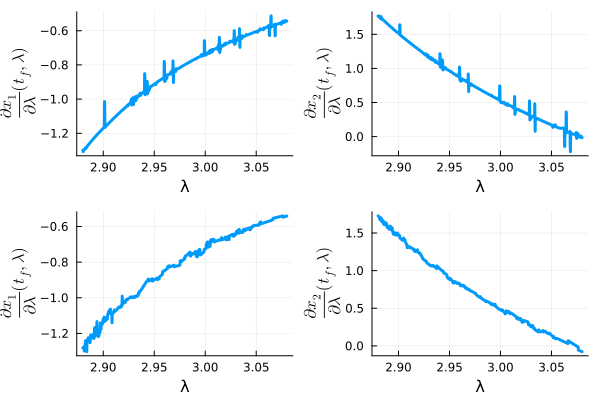
\includegraphics[width=\sizeFig\textwidth]{./figures/plot_END.png}

    \caption{Derivative computing by finite differences. $t_f=20, \lambda$ ranging from 2.88 to 3.08, $Tol=RelTol=AbsTol=10^{-4}$. Top graphs is for  $\delta\lambda=4Tol$ and bottom graphs for $\delta\lambda=\sqrt{Tol}$. The numerical integrattion is done with Tsit5().}
   % \label{fig:homotopy_epsilon_turnpike}
\end{figure}

\subsection{Variationnal equation }
Here the derivative $\frac{\partial x}{\partial \lambda}(t,t_0,x_0,\lambda_0)$ is the solution of the variational equation 
$$({VAR\ivpref\label{varlambda}})
\left\{\begin{array}{l}
\ddx(t)=A(t)\dx(t)+B(t)\\
\dx(t_0)=x_0'(\lambda),
\end{array}\right.
$$
with $B(t)=\frac{\partial f}{\partial \lambda}(t,x(t;t_0,x_0,\lambda_0),\lambda_0)\in\mathcal{M}_{n,p}(\IR)$.

\begin{figure}[ht!]
    %\centering
    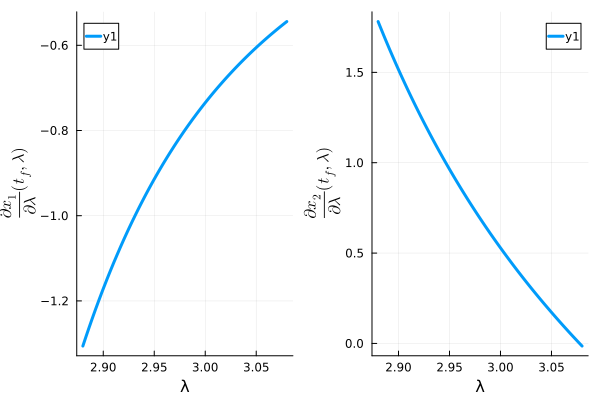
\includegraphics[width=\sizeFig\textwidth]{./figures/plot_var1.png}

    \caption{Derivative computing with the variational equation. $t_f=20, \lambda$ ranging from 2.88 to 3.08, $Tol=RelTol=AbsTol=10^{-4}$.  The numerical integrattion is done with Tsit5().}
   % \label{fig:homotopy_epsilon_turnpike}
\end{figure}

\begin{rmq}{Différentiation interne de Bock}
We can also approximate $A(t)$ and $B(t)$ by finite difference. But know, as we can use automatic differentiation for computing them, we don't  test this possibility. 
%On a 
%$$\vec{H}(t,z(t)+\eta \delta z_j(t))=\vec{H}(t,z(t))+\frac{\partial \vec{H}}{\partial z}(t,z(t))\eta \delta z_j(t)+o(\eta \delta z_j(t))$$
%On approxime alors dans les équations variationnelles
%$$\frac{\partial \vec{H}}{\partial z}(t,z(t))\delta z_j(t)\approx
%\frac{1}{\eta}(\vec{H}(t,z(t)+\eta \delta z_j(t))-\vec{H}(t,z(t))).$$
%On résout donc
% $$
%(IND_j)\left\{\begin{array}{l}
%\dot{z}(t)=\vec{H}(t,z(t))\\            
%\dot{\delta z}_j(t)=\frac{1}{\eta}(\vec{H}(t,z(t)+\eta \delta z_j(t))-\vec{H}(t,z(t)))\\
%z(0)=z_0\\
%\delta z_j(0)=e_j.
%\end{array}\right.$$
\end{rmq}

\subsection{Automatic differentiation of the flow}

Here, we use automatic differentiation on the function $\vphi(\lambda) = x(t_f,t_0,x_0(\lambda),\lambda)$. This is also known as the Internal Numerical Differentiation of  Bock \cite{Bock81}

\begin{figure}[ht!]
    %\centering
    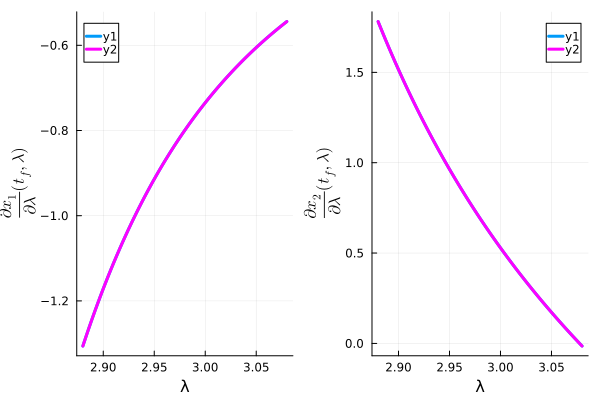
\includegraphics[width=\sizeFig\textwidth]{./figures/plot_diff_flow1.png}

    \caption{Derivative computing by automatic differentiation of the flow. $t_f=20, \lambda$ ranging from 2.88 to 3.08, $Tol=RelTol=AbsTol=10^{-4}$.  The numerical integrattion is done with Tsit5(), the automatic differentiation is ForwardDiff.}
   % \label{fig:homotopy_epsilon_turnpike}
\end{figure}

\section{Tests on the time steps}











%------------------------------------------------------------------------------------------------------------------
\section{Conclusion and perspectives}


% --------------------------------------------------------------------------------------------------------------------
\bibliographystyle{plain}
\bibliography{./main} 


\end{document}


